% -*- coding: utf-8 -*-
%%
%%  本模板可以使用以下两种方式编译:
%%     1. PDFLaTeX
%%     2. XeLaTeX [推荐]
%%  注意:
%%    1. 在改变编译方式前应先删除 *.toc 和 *.aux 文件,
%%       因为不同编译方式产生的辅助文件格式可能并不相同。

\documentclass{cumcmart}
% \documentclass[nocover]{cumcmart}%%%切换到无封面的版本,有些区域不允许前面的承诺页用pdf格式,可以用此去掉。



\begin{document}

\xuanti{A}
%\school命令用于在承诺书上显示学校名称。按要求,此处应填写全称
\school{长江大学}
%以下命令分别显示队员及指导教师姓名
\numbers{2017000}%参赛报名号
\authorone{成员一}
\authortwo{成员二}
\authorthree{成员三}
\advisor{数模指导组}

%\theyear{2017}
\theday{20}%填写当月的具体日期

\title{Title}

\maketitle

\begin{cnabstract}%此处没有采用sbstract命名,是为了将来如果要加入英文摘要时扩展的方便


\cnkeywords{差分方程,元胞自动机,交通阻塞模型,数值模拟}
\end{cnabstract}

\newpage
%\tableofcontents\newpage%增加目录,要不要都可以。不想要的话,就在本行前加“%”(英文的百分号)


\section{问题重述}


\section{建模分析}

\subsection{模型假设}
针对该模型,我们提出了如下的合理假设:
\begin{enumerate}
\item 
\item 
\item 
\item 
\end{enumerate}

\subsection{记号说明}
\begin{table}[!htbp]
    \centering
    \begin{tabular}{cl}
    \toprule
    \multicolumn{2}{c}{\large 模型记号说明}\\
    \midrule
    ${c_{ij}}$ &  i产品在j设备上加工的件数 \\
    ${e_{ij}}$ &  i产品在j设备上加工所需要的工时 \\
    ${a_i}$    &  i产品每件获得的利润 \\
    ${b_j}$    &  j设备最大负荷工时 \\
    ${d_j}$    &  j设备满负荷时需要的费用 \\
    \bottomrule
    \end{tabular}
    \caption{模型记号说明}
\end{table}

\subsection{建立模型}

    
    \[ %\begin{equation}
    s.t.
    \left\{  
    \begin{array}{ll}  
    \sum\limits_{i=1}^{2}{c_{ij}} = \sum\limits_{i=3}^{5}{c_{ij}} & j  = 1,2,3  \\ 
     \sum\limits_{i=1}^{3}{c_{ij}e_{ij}} \leqslant b_{i} & i = 1,2 \cdots 5 \\
    \end{array}  
    \right.
    \] %\end{equation} 

\subsection{模型求解和分析}
 

\subsection{模型评价}
\subsubsection{模型优点}
1)	

2)	

3)	

\subsubsection{模型缺点}
1)	

2)	


%   \begin{figure}
%   \centering
%   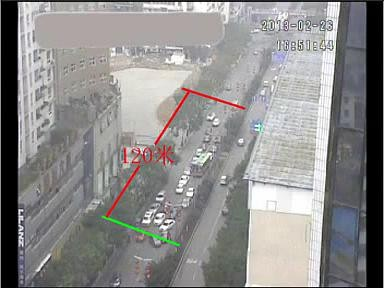
\includegraphics[width=.6\textwidth]{fig1}
%   \caption{发生事故时车流饱和状态图示}
%   \end{figure}

% \begin{thebibliography}{10}
% \bibitem{1} \url{http://bbs.chinatex.org}
% \bibitem{2} \url{http://www.chinatex.org}
% \bibitem{3} Alpha Huang, \textbf{latex-notes-zh-cn}, 2014.
% \bibitem{lf}M.R.C. van Dongen,\textbf{\LaTeX-and-Friends}, 2013.
% \bibitem{figure}Keith Reckdahl,\textbf{Using Import graphics in \LaTeXe}, 1997.
% \bibitem{HM}Addison Wesley,\textbf{Higher Mathematics}, 下载地址如下\\ \url{http://media.cism.it/attachments/ch8.pdf}
% \end{thebibliography}


\newpage
\appendix
\section*{附 \quad 录}


\end{document}
